
% !TeX spellcheck = en_GB
% Template for ICASSP-2010 paper; to be used with:
%          mlspconf.sty  - ICASSP/ICIP LaTeX style file adapted for MLSP, and
%          IEEEbib.bst - IEEE bibliography style file.
% --------------------------------------------------------------------------
\documentclass{article}
\usepackage{amsmath,graphicx,02460}
\usepackage{url}
\usepackage{mathtools}
\usepackage{booktabs}
\usepackage{caption}
\toappear{02456 Deep Learning, DTU Compute, Autumn 2019}
\newcommand{\pro}{\ensuremath{\ \%}}

% Example definitions.
% --------------------
\def\x{{\mathbf x}}
\def\L{{\cal L}}
\usepackage{fancyhdr}
\pagestyle{plain}

% Title.
% ------
\title{SegNet on Drone Images: Image Segmentation for Smart Agriculture}
%
% Single address.
% ---------------
\name{			Anders Henriksen, Asger Schultz, Oskar Wiese, 	Mads Andersen,
	Søren Winkel Holm }
\address{\{s183904, s183912, s183917, s173934, s183911\}@student.dtu.dk}
%
% For example:
% ------------
%\address{School\\
%	Department\\
%	Address}
%
% Two addresses (uncomment and modify for two-address case).
% ----------------------------------------------------------
%\twoauthors
%  {A. Author-one, B. Author-two\sthanks{Thanks to XYZ agency for funding.}}
%	{School A-B\\
%	Department A-B\\
%	Address A-B}
%  {C. Author-three, D. Author-four\sthanks{The fourth author performed the work
%	while at ...}}
%	{School C-D\\
%	Department C-D\\
%	Address C-D}
%
\begin{document}
%\ninept
%

\maketitle
%
\begin{abstract}
Identifying crops, weeds and unplanted dirt in a field is a major task in agriculture and the identification is crucial when making decisions about fertilization and pesticides.
A solution to the image segmentation task where the goal is to classify the locations  of crops, weed and soil based on drone images of a field, can speed up and improve this time consuming task for a farmer. 
In this paper, we solve the problem with Deep Learning, presenting an implementation of the deep neural network: SegNet and a strategy for training.
The purpose is to build an efficient deep neural network: both memory and time wise during inference. 
The architecture consists of an auto-encoder format, where max-pooling indices are used as skip connections.
%To show the efficiency of SegNet, a brief comparison of SegNet and other leading image segmentation architectures is included. 
%The comparison focuses on the trade-off between memory usage and accuracy and shows that with half the memory usage during inference SegNet only has a slight loss of accuracy.
To expand the limited data set several data augmentation techniques is used to improve the training of the network and a number of classic deep learning regularization techniques help with segmenting a sugar cane field from Brazil.
In conclusion, the deep network is able to classify the crops, weed and soil and obtains a F1-score at $ 85 \% $ with low overfitting which we attribute to the data augmentation.
It is found that using frequency weighted cross entropy loss for training is crucial for this class unbalanced data set and that this direct method does not sustain its' performance on a significantly smaller data sets. 
\end{abstract}
%
\begin{keywords}
Machine learning, Deep learning, Image Segmentation, SegNet, Smart agriculture, Drone imaging, Precision agriculture, Computer vision
\end{keywords}
%
\section{Introduction}
\label{sec:intro}

\subsection{Deep Learning and Precision Agriculture}
Image segmentation and object classification have received a lot of attention in recent years.
This is partly due to the wide array of possible applications and the recent interest in machine learning and, in particular, deep learning.
One such important application is separating weeds, crops and dirt in aerial drone images of a field. Applying the SegNet architecture to this field of crop segmentation could open up for smart agriculture that allows a farmer to localize the use of fertilizer and pesticides with positive environmental and economic consequences.
Using the deep learning architecture \textit{SegNet} for this classification could prove useful in terms of the computational efficiency, as this more memory efficient model allows for end-to-end training and makes embedded systems, e.g. in drones, feasible.

\subsection{Challenges of Image Segmentation}
Accurate image segmentation has been pursued for a number of computer vision, tasks including medical images and autonomous vehicles \cite{seg}.
Here, the typical problems include the classic deep learning challenge of generalizability as the training of the deep networks must converge to a  model which is robust to the variance in the population of images.
In computer vision, this is particularly challenging as photographic data has a notorious \textit{long tail} of rare images in the image population which challenges the generalizability model and must be addressed by regularization in multiple forms \cite{long}.   

In image segmentation, this problem of robust, generalizable models can be even more difficult as the classes that are to be predicted often have very different frequencies of occurence: Some -- often background classes like \textit{dirt} in this task -- are very prevalent while other classes appear rarely among the pixels but are still important to the task. 
This imbalance must be addressed in the training and evaluation for effective segmentation also for this task which contains 3 classes: \textit{weeds}, \textit{crops} and \textit{dirt}.

\subsection{The Data: Brazilian Sugar Canes and Danish Corn}
The primary data set in question consists of two large, high resolution orthomosaic RGB images of a Brazilian sugar cane field\footnote{Aerial image: http://www.lapix.ufsc.br/wp-content/uploads/2019/05\\/sugarcane2.png\\
Ground truth: http://www.lapix.ufsc.br/wp-content/uploads/2019/05\\/crop6GT.png} \cite{brazil}.
The first image consists of several drone images stitched together, with the second image of the same size being the manually labelled human ground truth, labelled by an expert biologist.
The three classes each have a corresponding colour -- crop rows are green, weeds are yellow, and soil is red.
Void pixels (not part of the field) are black.

We also used a second, smaller data set from a Danish corn field. This data set consists of already cut-out images: 20 for training and 4 for testing.
We did not use this for hyper parameter optimization or architectural decisions like this primary dataset.
Instead, only a train/test split was used to evaluate the network using the exact same hyper parameters. 




%In the following segments of this paper, the relevant methods, results and discussion will be covered; In section 2, methods such as regularization, data augmentation, metrics and chosen loss function are described. The results are tabulated in section 3. Section 4 is a discussion of the results and accuracy of the reconstruction, a comparison to other similar methods as well as a perspective on the problem. The relevant references are included in section 5.

\section{METHODS}
\label{sec:format}
\textit{All code is available at \url{github.com/sorenmulli/alpha_cellari_imageseg}. To reproduce the main results, the Jupyter Notebook} \texttt{image-segmentation.ipynb} \textit{from the folder \texttt{/src} can be run.}
\subsection{Preprocessing and Data Augmentation}
In order to use a deep neural network on the images and get the most effective learning out of the data, preprocessing is needed.
First, the RGB values of the non-void pixels of the aerial image are standardized to zero mean and one standard deviation, and a matrix is used to represent the biologists' ground truth.
This target matrix has is set up such that each entry corresponds to a pixel in the image and contains the numbers 0, 1, 2 for the different classes in the task or 3 for a void pixel.
The images are then padded with black pixels and cropped into smaller $ 512\times 512 $ pixel images.
Any of these images containing only black pixels are discarded, leaving a total of 108 pairs of aerial photo/ground truth images.
These are then split into 69 training, 18 validation, and 25 test images.

In order to increase the effective size of the dataset, we perform aggressive data augmentation.
When training the network, each pair of aerial photo/ground truth images is randomly cropped into $ 350\times 350 $ pixel images.
Furthermore, we applied a 50\pro\ chance of performing a top/down flip as well as a 50\pro\ chance of left/right flip to each image pair.
Even though data augmentation is not as effective as more independent data, it is used as a form of regularization to avoid the network learning the particularities of the data.

The same preprocessing was applied to the secondary dataset with the only difference being that black pixels were a class, so these were not left out of the training and evaluation.
Here, we ended up with 20 train and 4 test images.
\begin{figure}[!h]
	\centering
	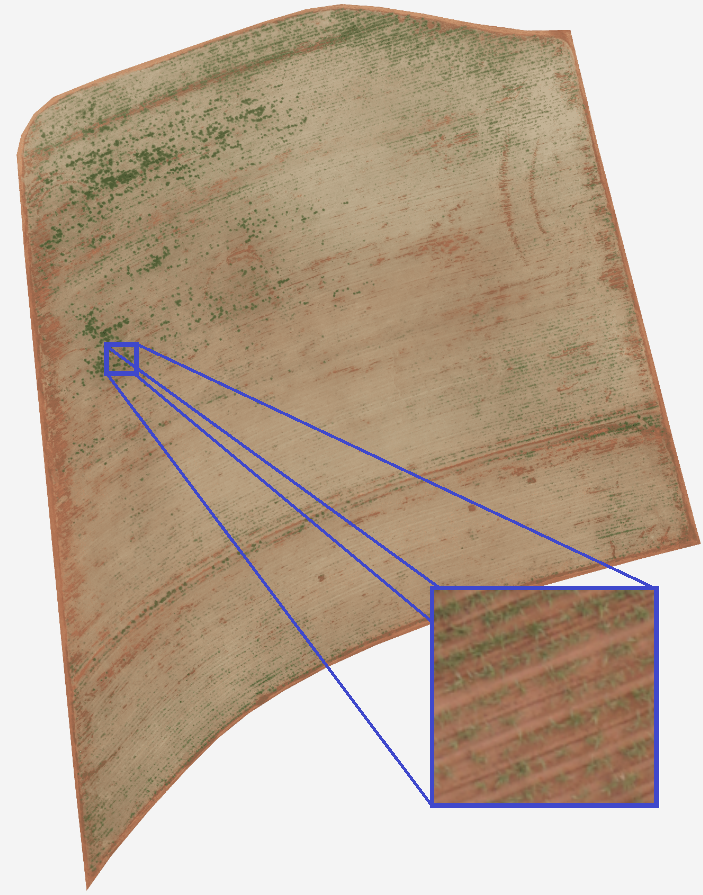
\includegraphics[width=0.5\linewidth]{../../poster/raw-min3}
	\caption{The main data set consists of this image of a Brazilian sugar cane field. The large image is cut into 112 \(512\times512\)-images with 69 used for training, 18 for validation and 25 for testing. }
	\label{fig:raw-min2}
\end{figure}

\subsection{The Model: SegNet}
%
The model used for this task is the Deep Neural Network SegNet which is built for Image Segmentation \cite{seg}.
The SegNet model architecture utilizes convolutional neural networks (CNN). 
CNN's work by convolving over an image with learned kernels which should correspond to features that are characteristic for the task.
The kernel size, stride and padding are all adjustable parameters that help to fit the kernel to a specific image dimension or, as in the case of SegNet, keep the dimensions of the image constant. 


%Encoder / Decoder  
SegNet's model architecture has an encoder-decoder structure. The encoder creates dense feature maps with the most vital information and by using max pooling layers achieves translational invariance over small spatial shift in the incoming image, and the decoder learns to upsample and seperate the classes.
The model consists of a total of ten blocks which either have two or three convolutional layers. Encoder blocks ends with a max-pooling layer whereas decoder blocks starts with an upsampling layer also called  un-pooling.
Every encoder and decoder block has applied Dropout for regularization, Batch Normalization for normalization of the activations, ReLU for non-linearity and Max Pooling for translational invariance.
The last layer is a softmax layer, which allows for probabilistic predictions from the model and evaluation of these. The dimensions of the encoder and decoder blocks are equal and mirrored. Thus, the input and output dimensions are the same as is needed for image segmentation where each pixel is to be classified.
\begin{figure}[!h]
	\centering
	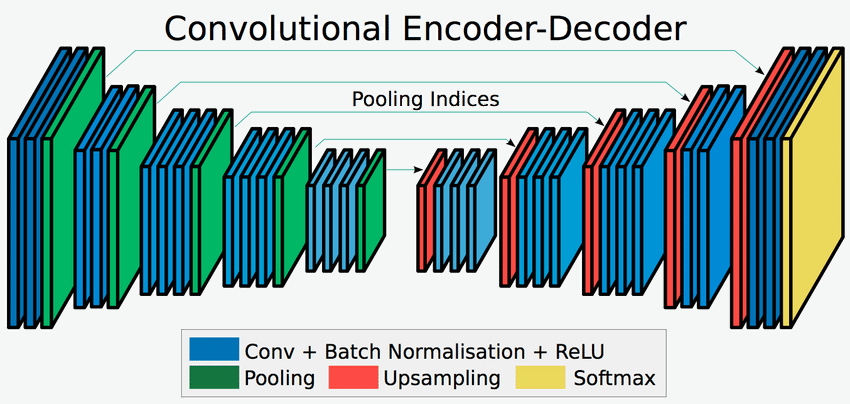
\includegraphics[width=0.8\linewidth]{../../poster/Encoder-Decoder2}
	\caption{Illustration of the SegNet architecture from \cite{seg}. Note that the mirrored structure allows for the input and output to have the same size which is appropriate for image segmentation.}
	\label{fig:encoder-decoder2}
\end{figure}
\\
%Skip connections 
The encoder part of the network creates a lower dimensional, but semantically richer feature map representing the image content but the boundary detail is very important when dealing with image segmentation.
Hence, it is beneficial to preserve the boundary information in the feature maps of the encoder before upsampling.
This can simply be done by storing the entire feature map in the encoder part and appending it to the decoder activations but this has the issue of being memory inefficient. 
Therefore, in SegNet, skip connections between each encoder and decoder block are introduced by storing only the max-pooling indices from each max-pooling layer. 
Upsampling is now performed by casting the decoder activations to the indices in the feature map corresponding to the encoder activations and leaving the rest of the positions in the larger feature map empty (zeros are used in this implementation) thus combining the information of the encoder and decoder when upsampling.

 \begin{figure}[htb!]
 	\begin{equation*}\label{key}
\scriptsize
\begin{bmatrix}a&b\\c&d\end{bmatrix} \xrightarrow{\text{\scriptsize M. pool indices}}
\begin{bmatrix}0&0&0&a\\b&0&0&0\\0&c&0&0\\0&0&d&0\end{bmatrix} 
\rightarrow 
\texttt{\scriptsize Conv2d}
\end{equation*}
 	\caption{An illustration of an example of upsampling using max pooling indices as skip connections corresponding to the red layers in figure \ref{fig:encoder-decoder2}. Note that activations from the decoder and positions from the encoder are combined to result in a sparse, upsampled feature map which is further propagated through the network.}
\end{figure}
\noindent 
It has been argued and exemplified in earlier tests, that storing the max pooling indices is a good approximation of the actual feature map  while being considerably more memory efficient \cite{seg}. 



\subsection{Regularization: Dropout and Batch Normalization}
Because deep neural networks are such highly flexible models, regularization is necessary on top of the data augmentation to further reduce overfitting.
This is done in two ways.

Dropout at 10\pro\ is used after each blue block in the network (see Fig. \ref{fig:encoder-decoder2}).
This procedure randomly shuts off nodes during training leading to node redundancy and variability, as the same input will vary somewhat in its output, which forces the network to be more robust.
We experimented with higher dropout, but found that too high values would significantly reduce learning.

Batch normalization is applied after each dropout.
This standardizes the activations, keeping them close to zero.
As a result, the weights and biases also stay close to zero, which reduces the flexibility of the model, leading to less overfitting.
Batch normalization also has several other benefits, such as reducing the vanishing gradient problem and allowing for a higher learning rate and thus faster convergence time \cite{bn}. 

\subsection{Training: Learning from Quality over Quantity}
For training -- finding the optimal weights of the network -- the widely used Adam optimizer  was implemented because the addition of momentum to the efficient and effective Stochatic Gradient Descent algorithm is shown to giver faster convergence in a wide range of computer vision tasks \cite{Adam}. The training was done in 3000 epochs each consisting of mini batches of size 3.

A less obvious choice was the loss function. It was clear that 3-class cross entropy should be used for criterion as this, for a Softmax network such as SegNet, can be seen as following the maximum likelihood principle and implementing minus logarithmic likelihood loss. The direct implementation of this, however, failed to consider a deep issue in Image Segmentation which had considerable effect on this limited data set: \textit{class imbalance}. 
In the main data set, there is \(\sim 93 \%\) pixels belonging to the \textit{dirt}-class which arguably is the least interesting and initial tests saw the network behave too much as a baseline; simple features in early layers which classified almost everything as dirt were not penalized enough and learning was not stable. 

As resampling an image data set is computationally expensive and it was desired that the network learned to focus on important pixels, it was chosen the main training experiment of this report should use \textit{weighted cross entropy} where each class is weighted by \(w_i = 1-\nu_i\) where \(\nu_i\) is the frequency of class \textit{i} thus focusing more on the classes crops and weeds than in the vanilla cross entropy. The implemented loss of \(N\) pixels in a one-hot encoded \((N \times  3)\) output matrix \(\mathbf X^\text{pred}\) with the true classes \(\mathbf c\) was then:
\[
L = \underbrace{
	\vphantom{\sum_{i}}
	\frac 1 N
	\sum_{\mathclap {i=1}}^{N}
}
_{\mathllap{\text{Mean over minibatch}}}
\underbrace{ 
	\vphantom{\sum_{i}}
	\mathbf{w}[i, c_i]}
_{\mathclap{\text{Class weight}}}  
\cdot 
\underbrace{
	\log 
	\frac
	{-\exp\mathbf X^\text{pred}[i, c_i]}
	{\sum_{j=1}^{3}\exp\mathbf X^\text{pred}[i, j]}
}_{\mathclap{\text{3-class cross entropy}}}
\] 
To test the importance of this frequency balancing for this data set, another training experiment was set up without weighting of the cross entropy loss.
\subsection{Evaluation Metrics: Finding the Important Story}
In the compared image segmentation literature no single accuracy measure can be described  as the canonical metric resulting in a number of metrics being compared \cite{eval, Metric}.  A collection of different metrics are usable as the performance of the image segmentation both the global and the local scale is relevant. 
%	\item Different metrics important in different fields.
Four simple accuracy measures are used here to mirror the SegNet paper \cite{seg} though more complex measures which fit better with human evaluation exist \cite{eval}. 

The simple global accuracy, the frequency of correct classifications, is not the most meaningful measure for class imbalanced data sets such as this (the baseline achieves \(>90\%\) on this metric) but is in the literature noted to be important for a smooth classification \cite{seg}. Another simple measure is the mean of the accuracies of model on the three classes. This measure is still a naïve accuracy measure but is the metric which is being optimized for in the weighted cross entropy loss. 

The metric which is being seen as the main performance metric is the F1-score: The harmonic mean of precision of recall. This is used for comparison to other groups with same project and because this metric penalizes false positives and gives less credit to true negatives thus being better for unbalanced classes \cite{Metric}. A related score is the Mean Intersect over Union (MIoU), also known as the Jaccard Index, which penalizes false positives harder and is found to be better correlated to human evaluation though only \(\sim 0.5\) \cite{eval}. 

Both F1 and MIoU are calculated for each of the three classes and are then averaged to get the final score. Both of them favour region smoothness higher than boundary accuracy compared to semantic accuracy measures such as the Berkeley contour matching score \cite{seg}.

To estimate generalization performance, the models are compared by their performance on the \textit{test data set} which is kept separate from the training and validation data and is pre-divided for both data sets consisting of approximately \( 20\%\) of the images.  It is noted that this simple hold out evaluation method does not claim to give an accurate estimate of generalization error on \textit{any} data set but can statistically only be seen as an evaluation of the performance on the used data sets. 

\subsection{Three Experiments and Their Hyper Parameters}
When training the network, we used the following hyperparameters: Batch size of 3, dropout of 10\pro, and a learning rate of $ 1.5\cdot 10^{-4} $ with the ADAM optimization algorithm.
For the convolutional layers, kernel size was set to $ 3\times 3 $ and stride to $ 1 $, as deeper network structures with smaller kernels tend to learn to better and faster.
This is because the receptive field is the same as larger kernels in shallower networks, but the multiple layers allow for learning more complex structures.
In the encoder part, the first convolutional layer increased the number of channels to 64.
Thereafter, the first convolutional layer in each block doubled the number of channels, ending at 512.
In the max pooling layers, we used a $ 2\times 2 $ with a stride of 2, cutting the size of the feature maps to a quarter each time.
The decoder part exactly mirrored this structure.

Three experiments with these hyper parameters were run: One called the \textit{main} experiment was run using the Brazil Sugar Cane data set and the class frequency weighted cross entropy loss.  The second was run with the same data and hyper parameters but with vanilla cross entropy loss to test the effect of class frequency balancing. The third was run with the same hyper parameters and class frequency weighting but using the smaller Danish Corn data set.

The training can be recreated using the Jupyter Notebook at \texttt{src/image-segmentation.ipynb} folder in the Github repository.
Because training the network takes close to 30 GB of VRAM, we have implemented a simpler version of SegNet with fewer layers that takes significantly less memory to train.
This is controlled using the \texttt{use\_simple} variable, which is set to \texttt{True} by default.


\subsection{Unification of Cropped Image Predictions}
In a real-world application of field classification a farmer would want a complete and precise segmentation of the whole field at once such that fertilizer and pesticides can be distributed accordingly.
To accomplish this, a reconstruction of the 112 smaller image inferences into a large image is necessary.
The most straight forward method of combining the smaller images is by lining them up next to each other.
This reconstruction method results in a very rough transition between the smaller inferences. An illustration of this can be seen in the left side of figure \ref{fig:earlylatereconstruction}.
The blocky nature of the field prediction is caused by a lack of information from neighbouring pixel, when inference is performed near the borders of an image. 
To solve this problem, the cropping size of the field into smaller images is increased and some overlap is added. This corresponds to adding padding pixels from the original field.
In the procedure of joining the enlarged images they are cropped again, to avoid the border areas. At the cost of computational efficiency more information is available near the borders and a smooth transition between the smaller inferences can be achieved. This can be seen in the right side of figure \ref{fig:earlylatereconstruction}. A visualization of the reconstruction technique can be seen in appendix \ref{reconstruction_technique}.



\begin{figure}[!htb]
	\centering
	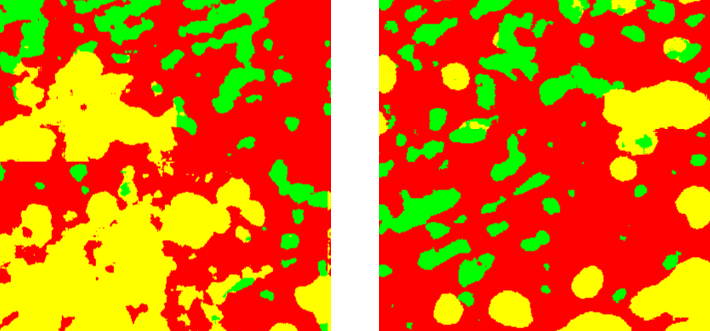
\includegraphics[width=0.9\linewidth]{early_late_reconstruction2}
	\caption{\textbf{Left:} Smaller inferences put next to eachother without use of reconstruction techniques. \textbf{Right:} Reconstruction with padding and overlap between smaller inferences. Note that the border between the four images is visible in the left image but not in the right.}
	\label{fig:earlylatereconstruction}
\end{figure}





\section{RESULTS}
\label{sec:illust}

\begin{table}[!htb]
	\centering
	\begin{tabular}{l r r r r}
		\textbf{Train results} & & & & \\
		\toprule
		Method  &  G.acc.  &  C.acc.  &  Mean IoU  &  F1 \\ \midrule
		Baseline  &  0.91  &  0.33  &  n/a  &  0.32 \\
		\textbf{Main SegNet}  &  0.97  &  0.90  &  0.80  &  0.88 \\
		Unweighted loss   &  0.96  &  0.71  &  0.66  &  0.78 \\
		\midrule 
		Corn Baseline  &  0.39  &  0.33  &  0.13  &  0.19 \\
		Corn SegNet  &  0.79  &  0.78  &  0.65  &  0.79 \\
		\bottomrule
	\end{tabular}
\end{table}

\begin{table}[!htb]
	\centering
	\begin{tabular}{l r r r r}
		\textbf{Test results} & & & & \\
		\toprule
		Method  &  G.acc.  &  C.acc.  &  Mean IoU  &  F1 \\ \midrule
		Baseline  &  0.94  &  0.33  &  n/a  &  0.32 \\
		\textbf{Main SegNet}  &  0.98  &  0.86  &  0.75  & \textbf{ 0.85} \\
		Unweighted loss  &  0.97  &  0.61  &  0.57  &  0.69 \\
		\midrule
		USC SegNet  &  n/a  &  n/a  &  0.79  &  0.96 \\
		USC UNet  &  n/a  &  n/a  &  0.75  &  0.93 \\
		Cellari DNN  &  n/a  &  n/a  &  n/a  &  0.88 \\
		\midrule 
		Corn Baseline  &  0.32  &  0.33  &  0.11  &  0.16 \\
		Corn SegNet   &  0.35  &  0.36  &  0.21  &  0.34 \\
		\bottomrule
	\end{tabular}
\end{table}
\noindent Above, the G.acc. refers to global accuracy, C.acc to class accuracy and F1 to the F1-score.

The baseline is construced by predicting most prevalent class.
USC is the first work on the data set from Universidad de Catarina \cite{brazil} and Cellari is the work from the project supervisor \url{cellari.io}.
Note that we don't have access to all accuracy measures for other implementations and, importantly, that the USC. implementations do not have the same train/test-split as the one used for this project.
\begin{figure}[!htb]
	\centering
	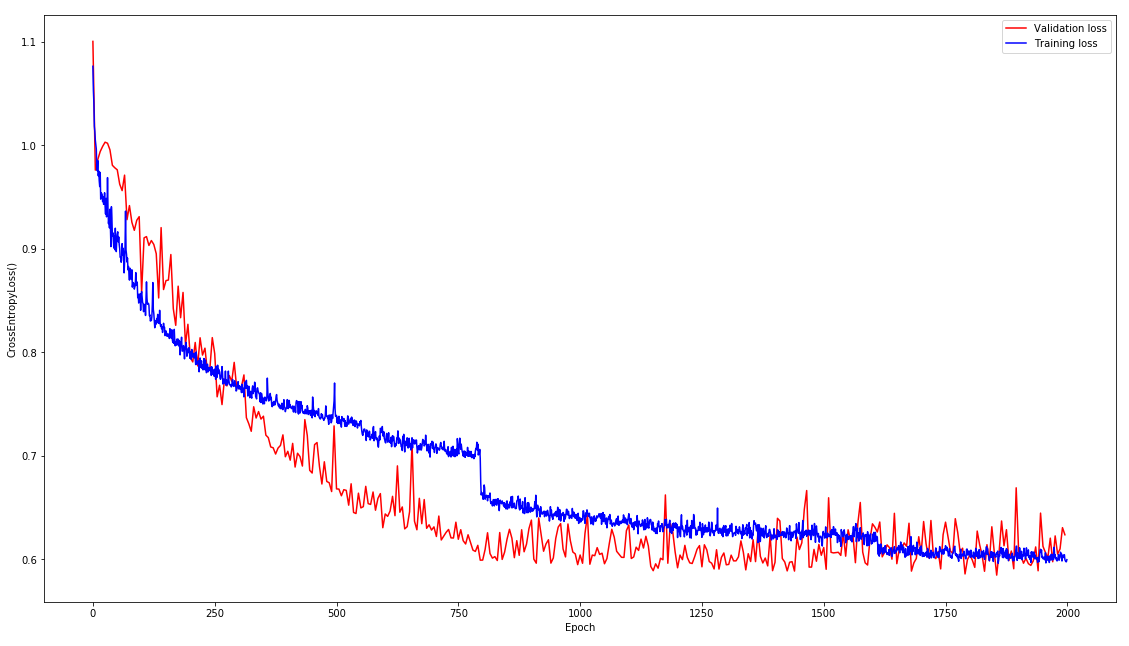
\includegraphics[width=0.9\linewidth]{../../poster/loss}
	\caption{The loss curve of the main SegNet implementation on the Brtazil data set with the blue curve corresponding to training loss and the red corresponding to validation loss. Both loss values are computed after each epoch and in {evaluation mode} (without the usual effect of Dropout and Batch Normalization). Note the low degree of overfitting and the relatively stable convergence. }
	\label{fig:loss}
\end{figure}


% STANDARD BASELINE, CELLARIO AND COMPARED RESULTS LIGGER STADIG I POSTER

%STANDARD

%2019-12-10 22:31:52.335662	Calculating train accuracy measures...
%2019-12-10 22:32:04.165629	Accuracy measures: Global acc.: 0.9706
%Class acc.: 0.8993
%Mean IoU.: 0.7967
%Bound. F1: 0.8818
%
%2019-12-10 22:32:04.167743	Calculating test accuracy measures...
%2019-12-10 22:32:08.005059	Test accuracy measures: Global acc.: 0.9768
%Class acc.: 0.8585
%Mean IoU.: 0.7541
%Bound. F1: 0.851

%SIMPLELOSS
%2019-12-11 01:20:01.124762	Calculating train accuracy measures...
%2019-12-11 01:20:12.598002	Accuracy measures: Global acc.: 0.957
%Class acc.: 0.7078
%Mean IoU.: 0.6629
%Bound. F1: 0.7789
%
%2019-12-11 01:20:12.599878	Calculating test accuracy measures...
%2019-12-11 01:20:16.252676	Test accuracy measures: Global acc.: 0.9653
%Class acc.: 0.6107
%Mean IoU.: 0.5737
%Bound. F1: 0.6922


%CORN BASELINE 
%2019-12-28 16:30:59.018404	Evaluating Baseline

%2019-12-28 16:31:05.300109	Training accuracy measures: Global %acc.: 0.3925
%Class acc.: 0.3333
%Mean IoU.: 0.1308
%Bound. F1: 0.1879

%2019-12-28 16:31:06.241630	Test accuracy measures: Global %acc.: 0.3193
%Class acc.: 0.3333
%Mean IoU.: 0.1064
%Bound. F1: 0.1613


%CORN RESULTS

%2019-12-28 18:57:27.694899	Accuracy measures: Global acc.: 0.7938
%Class acc.: 0.7819
%Mean IoU.: 0.6505
%Bound. F1: 0.7877
%

%2019-12-28 18:57:28.459897	Test accuracy measures: Global acc.: 0.3518
%Class acc.: 0.3556
%Mean IoU.: 0.2069
%Bound. F1: 0.3398


\section{DISCUSSION}

\subsection{Performance of Networks: Loss and Size matter}
The main performance benchmark for this test of the SegNet implementation is the test F1-score on the Brazil sugar cane data set: \textbf{85\%}.
This score is seen as acceptable as it reaches a score which generally seen as high for image segmentation where human agreement of segmentation is often limited \cite{eval}.  It also clearly outperforms the baseline score of 0.32 but fails to reach the performance of other Deep Neural Networks: The Cellari DNN and the Universidad de Catarina implementations are 3-11 \% points higher. 

These differences can be due to data augmentation practises and hyper parameter optimization as the hyper parameters for these implementations could not be accessed.
For data augmentation, this project chose to use flipping and random cropping heavily and the forceful croppings from 512x512 to 350x350 (effectively halving the number of pixels for each epoch) might have limited the learning of the model as less data was accessible for each parameter update. 

The motivation for this data augmentation choice was mainly because of computational limits in training but it also resulted in no discernable trace of overfitting as can be seen from figure \ref{fig:loss} and the minor differences in train and the limited differences in test and train results.

This indicates that controlling the size of random croppings is another regularization parameter usable for balancing the bias/variance-tradeoff of image segmentation tasks. For MIoU, the measure which is closest linked with human evaluation \cite{eval}, the differences between this reports' main network and the other implementations were more slight. 
\begin{figure}[h!]
	\centering
	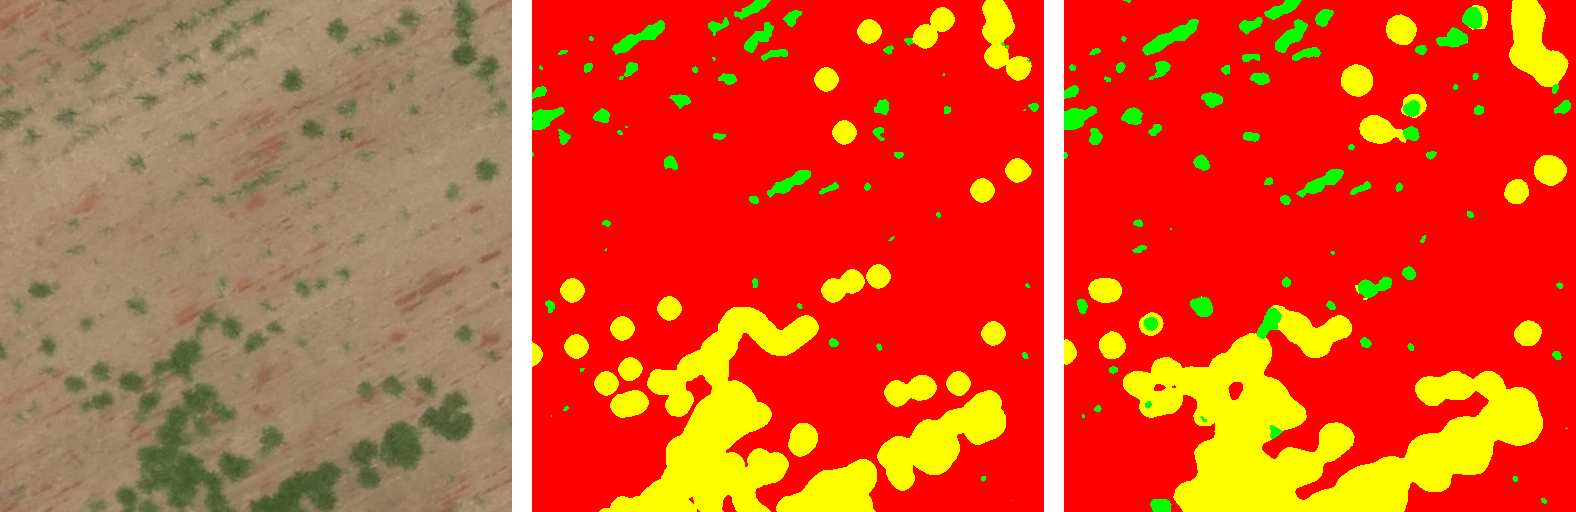
\includegraphics[width=\linewidth]{../../poster/reconst}
	\caption{An example of predictions. The true image (left) has a large portion of weeds (yellow) in the bottom and some crops (green) in the top as can be seen in the biologist ground truth (middle). The SegNet model recreates this test image well (right) but has some noise in the bulk of weeds and connects patches of plants too often. }
	\label{fig:reconst}
\end{figure}

\noindent
The test of the \textbf{loss function} gives clear results: The difference of 0.16 in test F1 score is assumed to be significant and the results for the unweighted cross entropy loss functions seem to fit the expected:
There is virtually no difference in the global accuracy -- for which the simple loss function optimizes -- showing that learning has occurred.
The large differences in the class-balanced accuracy measures indicate that, when all classes are of importance, the frequency weighted cross entropy loss should be used  for unbalanced data.
\\
\\
The test of the performance of the same, main SegNet model on the small, novel \textbf{corn field data} set gives disappointing results: Only a test F1 score of 0.34 which outperforms the baseline but tells a story of overfitting with a train F1 of 0.79 on this small data set of 20 512x512 train images.
 The data augmentation technique of heavy random croppings does not have the same regularizing effect on such a limited data set. 
Another problem might be that the cornfield data has a much nearer zoom level than the main sugar cane field.
This might not fit well with the model's field of view which is partially a product of the choice of kernel size of 3x3, max pool of 2x2 and other hyper parameters. Examples of images of the cornfield can be seen in the appendix in figure \ref{fig:corn} and can be compared to the left image in figure \ref{fig:reconst}.

\label{sec:foot}
\subsection{Comparison of Different Image Segmentation Neural Networks}
In the field of image segmentation there are several different neural network architectures that excel in different types of problems. Among the most acknowledged architectures are U-net, DeepLabv1, DeconvNet and FCN. 
All of these networks differ in several ways and it is important to emphasize that each network is designed to excel in a specific branch of image segmentation. U-net is as an example designed for medical image segmentation, whereas SegNet is designed such that it can be used in embedded systems. Each branch of problems has its own challenges and limitations. Therefore it is necessary to apply problem-specific methods to optimally segment the images. 
As mentioned earlier the purpose of SegNet is to be efficient in inference time and memory-wise, such that it can be used in embedded systems. And these two aspects are the ones we are interested in comparing SegNet and the other architectures. 
SegNet and its competitors have a quite similar performance in terms of accuracy on both road map scenes and the benchmark dataset known as SUN RGB-D, which is an indoor scene segmentation challenge \cite{seg}. 
With respect to the architecture all of these networks have a general structure like the one SegNet has with both an encoder and a decoder. The encoder of the competing networks (SegNet and three of the four competitors FCN, DeconvNet, U-net) have an almost topologically identical encoder, which originates from the well known VGG16 network \cite{VGG16}. One important difference between SegNet and the three other networks is that SegNet is without the final fully connected layers of the original VGG16 network, which decreases the amount of trainable parameters with almost 90\% \cite{seg}. 
All of the networks differ in decoding structure and techniques that is applied, and as a common denominator for FCN, DeconvNet and DeepLab-LargeFov they use nearly twice as much memory during inference. Among the heavy users of memory are the fully connected layers of the DeconvNet and FCN, and the full resolution feature maps that is used as skip connections in the U-Net. In comparison with the same 3 structures SegNet come in second only bested by DeepLab-LargeFOV with respect to inference time.


The encoder part of the network has only 14.7 million parameters compared to partially fully connected structures that tend to have well over 100 million. \cite{seg}


\subsection{Potential in SegNet}
The architecture of SegNet allows for an easy and fast end to end training of the network. As a consequence of this SegNet is easily modified into other use cases without much technical effort. Because of the low memory usage and the speed of which the inference takes place SegNet could prove to be a good choice for self-driving cars and drones. However, it can be challenging and costful to acquire labelled data as this typically involves professionals manually doing the labelling. In our project we only have a single field image, which is not representative of similar fields under different circumstances such as lighting, type of crop and season. The best way of increasing the robustness is to expand the data set, but another cheaper method is by using different augmentation techniques. There exits a vast amount of different techniques and some have proved useful to some problems whereas other augmentation are preferred in other problem settings. For this project random cropping, flipping have been used to increase robustness.

\subsection{Extension of network}


\subsection{Conclusion}
The purpose of this project has been to build an efficient neural network architecture for semantic pixel-wise segmentation on a crop field. The neural network implemented goes under the name SegNet, and it has been designed to be efficient in terms of memory usage and time during inference, such that it can be used in embedded system. The architecture consists of an encoder and a corresponding decoder network and ends with a pixel-wise classification layer. The purpose of the encoder is to reduce the dimensionality and extracts the useful information in the image thereby creating a dense feature maps that can be classified. This procedure is performed by using blocks of convolutional layers, each block ending with a max pooling layer. The decoder has to upsample the low-resolution feature map back into full input resolution, such that a precise pixel-wise classification can take place. During the encoding procedure only the most characteristic information is extracted with max pooling layers, and local information is lost. This local information is necessary for a precise classification and therefore SegNet uses max-pooling indices as skip connections to retain this local information. During the upsampling these max pooling indices are used to create a sparse feature map and afterwards convolutional layers are use to create more dense feature maps. The use of max pooling indices are a very efficient way of storing local information with only a slight loss of accuracy. Our results show that ------xx----. Conclusion ----x----.


\bibliographystyle{IEEEbib}
\bibliography{refs}
\subsection{Appendix}
\begin{figure}[h!]
	\centering
	\includegraphics[width=0.7\linewidth]{"reconstruction DL"}
	\caption{Reconstruction of the smaller inferences into a unified field prediction.}
	\label{reconstruction_technique}
\end{figure}

\begin{figure}[h!]
	\centering
	\includegraphics[width=0.7\linewidth]{"corn.JPG"}
	\caption{Example of a training image from the smaller Danish cornfield data set}
	\label{fig:corn}
\end{figure}

\end{document}




